\chapter{Resultados}

Se  puede afirmar que llegados a la finalización del desarrollo del sistema se ha obtenido un resultado satisfactorio. Se han implementado casi todos los requisitos del sistema y el videojuego provee de una experiencia de juego completa.

Se ha completado también el objetivo principal del proyecto: crear un videojuego que eduque sobre emprendimiento y \textquote{LeanStartup}. Se ha usado el storytelling para que el jugador reciba información sobre \textquote{Lean startup} al conversar con los NPCs del juego (ver fig. \ref{dialogo}).

\begin{figure}
\begin{center}
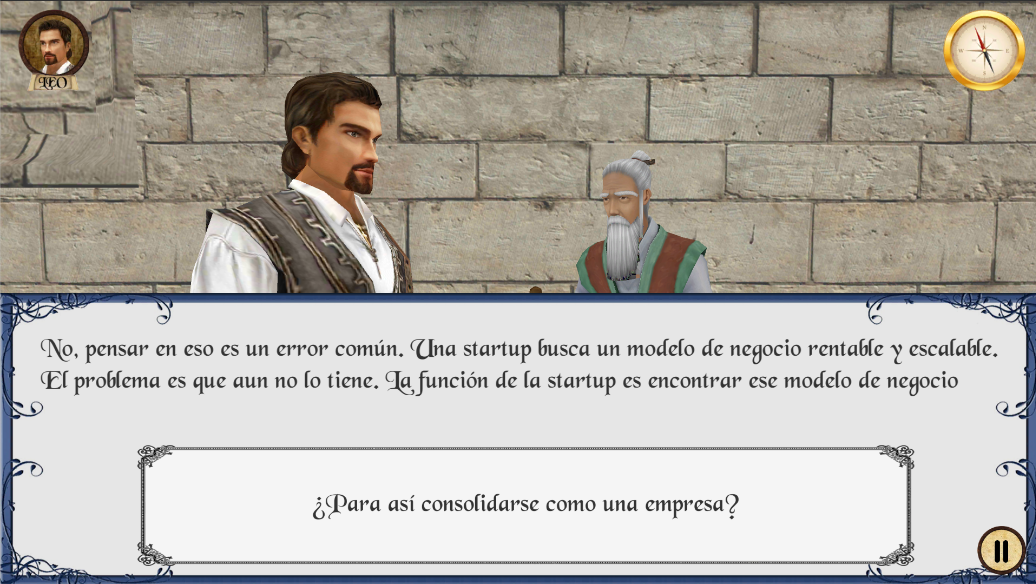
\includegraphics[scale=0.5]{imagenes/dialogo.png}
\caption{Jugador dialogando con NPC en Da Vinci Startu.  Fuente: elaboración propiap}
\label{dialogo}
\end{center}
\end{figure}

El desarrollo del proyecto se ha llevado a cabo con Unity3D y utilizando el lenguaje de programación C\#. Se han ampliado enormemente los conocimientos sobre ambas herramientas y se han aprendido muchas técnicas de desarrollo sobre las mismas.

Se han creado también varios  escenarios por los que el jugador puede transitar libremente y moverse de uno a otro(ver fig. \ref{escenarios}).

\begin{figure}
\begin{center}
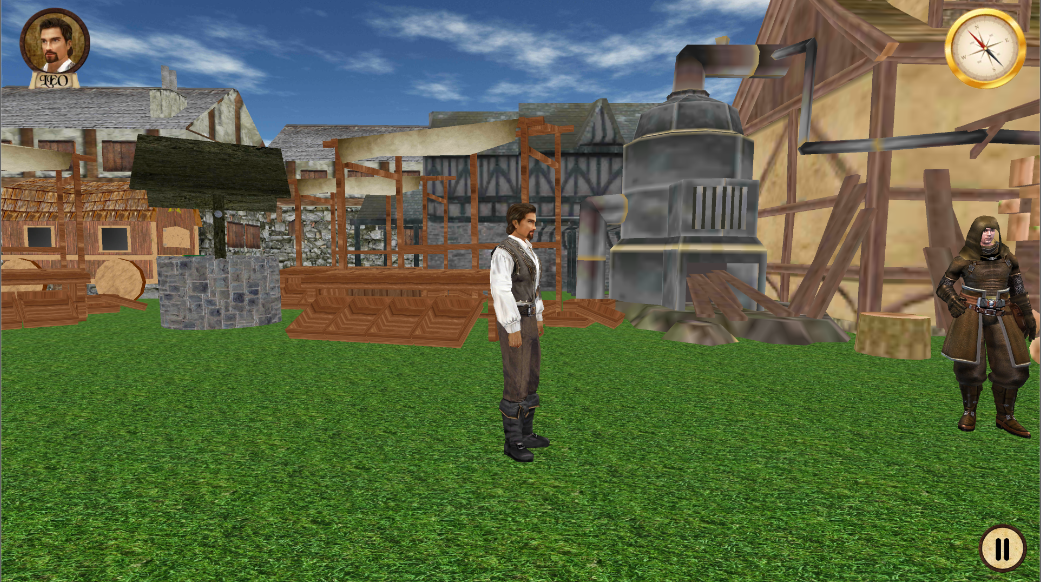
\includegraphics[scale=0.5]{imagenes/escenarios.png}
\caption{Jugador en el escenario Calles de Florencia}
\label{escenarios}
\end{center}
\end{figure}

Se ha implementado también el sistema de interfaces propuesto, ofreciendo al jugador  toda la funcionalidad necesaria pero sin comprometer la jugabilidad. Entre las interfaces creadas se encuentran  el selector de personajes, el indicador de objetivos y el menu de pausa (ver fig. \ref{iu}). Además se ha creado un menú principal con varias ventanas en las que visualizar información como los logros, las opciones, información sobre el desarrollador, etc (ver fig. \ref{titulo}).

\begin{figure}
\begin{center}
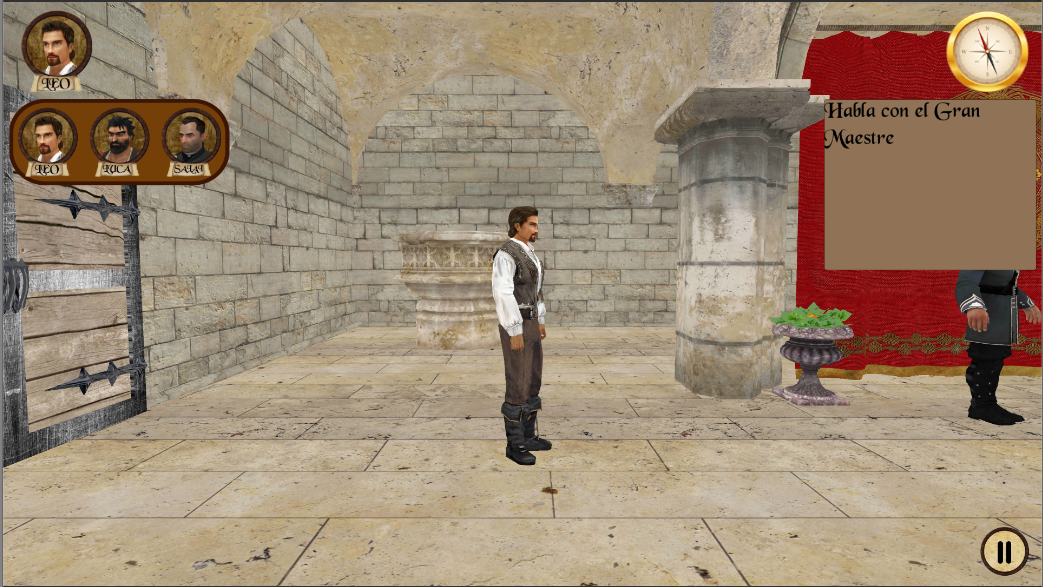
\includegraphics[scale=0.5]{imagenes/iu.png}
\caption{Interfaz de usuario durante la partida con los menús desplegados.  Fuente: elaboración propia}
\label{iu}
\end{center}
\end{figure}

\begin{figure}
\begin{center}
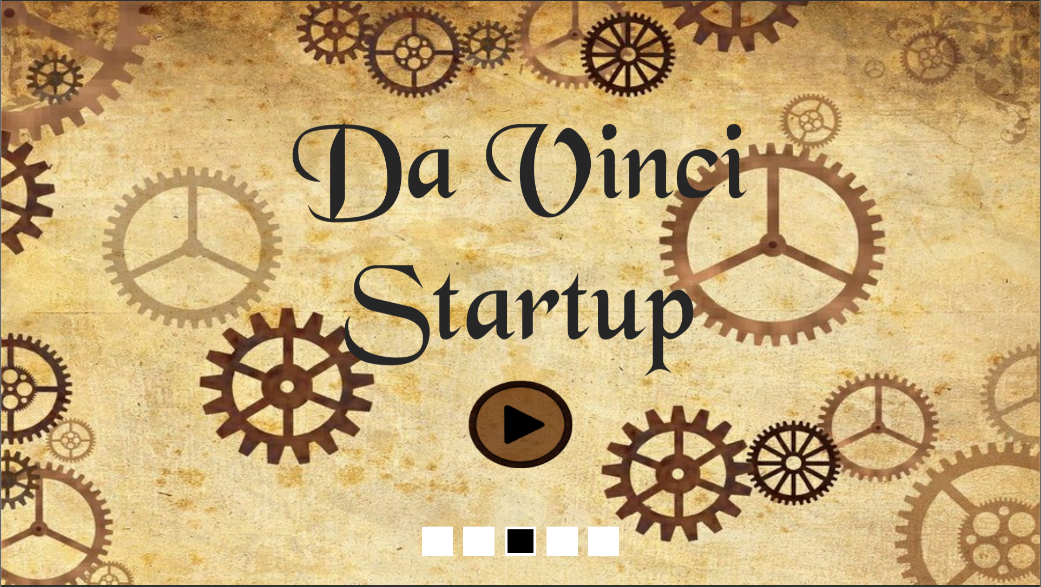
\includegraphics[scale=0.5]{imagenes/titulo.png}
\caption{Menú principal del juego.  Fuente: elaboración propia}
\label{titulo}
\end{center}
\end{figure}

En cuanto a los objetivos que no se han podido cumplir: no se han podido crear los modelos 3D para el juego. En su lugar se han tenido que utilizar recursos que se ofrecen de forma gratuita. Tampoco se han podido cumplir los requisitos correspondientes a Guardar juego (RF-SYS-08) y Cargar juego (RF-SYS-09). En cualquier caso no son requisitos que comprometan la experiencia de juego y que impidan el transcurso de una partida. 

En resumen, el producto creado no es un juego finalizado, pero si que se puede considerar un Mínimo producto viable que se podría enseñar a inversores que estén interesados en apoyar el desarrollo del juego. O mostrar a personas que podrían estar interesadas en unirse al equipo. También es el primer paso para poder probar el juego con usuarios reales y seguir trabajando acorde a las opiniones de estos. 

Para concluir, el producto creado cumple perfectamente con lo esperado del mismo. Ofrece una experiencia de juego completa y contiene todos los elementos planeados para el juego. Es un punto de partida perfecto para reunir un equipo, buscar financiación y convertirlo en un juego que se pueda comercializar.